%-----------------------------------------------------------------------------%
\chapter{LANDASAN TEORI}
%-----------------------------------------------------------------------------%
\vspace{4.5pt}
Pada bab ini menjelaskan beberapa teori dan jurnal yang berhubungan dengan permasalahan penelitian dan yang digunakan pada proses penelitian.
\section{Tinjauan Pustaka}
Pembahasan mengenai teori-teori tersebut akan dijelaskan sebagai berikut.
\subsection{Monolit}
Monolit yaitu suatu cara untuk melakukan penyebaran. Ketika semua fungsi dalam sistem harus disebarkan secara bersama-sama, maka itu merupakan monolit.\cite{6} Monolit merupakan sebuah aplikasi perangkat lunak dimana setiap modulenya tidak bisa dieksekusi secara independen. Hal ini membuat monolit sulit digunakan pada sistem terdistribusi tanpa bantuan penggunaan frameworks atau solusi ad hoc seperti Objek Jaringan, RMI atau CORBA.
Penggunaan pada bahasa utama seperti Java, C/C++, dan Python pada pengembangan aplikasi di sisi server. Memiliki kemampuan melakukan abstraksi untuk memecah kompleksitas program menjadi berupa modul. Namun, bahasa pemrograman ini dirancang untuk membuat artefacts monolit. Dimana abstraksi ini tergantung pada penggunaan berbagi sumber data pada komputer yang sama (memori, database, file).[?] 


Terdapat 3 jenis monolit \cite{6}:
\begin{enumerate}[leftmargin=1.3cm]
\item Single Process Monolith

Dimana sebuah kode disebarkan dengan satu proses. Dimana setiap kode bisa berada di banyak instances serta tempat penyimpanan dan mendapatkan data disimpan pada suatu database yang sama. Variasi lainnya yaitu modular monolith dimana setiap kode bisa bekerja secara independen tetapi perlu dijadikan satu kesatuan ketika ingin dilakukan penyebaran.
\item Distributed Monolith

Monolit terdistribusi adalah sistem yang terdiri dari beberapa layanan, tetapi untuk apa pun alasannya seluruh sistem harus disebarkan bersama-sama. Sebuah monolith terdistribusi mungkin akan memenuhi definisi dari sebuah arsitektur service-oriented (SOA).

Monolit terdistribusi biasanya muncul  di kondisi dimana tidak cukup fokus pada konsep information hiding dan kohesi dari fungsi bisnis. Akibatnya terbentuklah arsitektur yang memiliki kopel yang tinggi, dimana bisa perubahan menyebabkan kerusakan pada bagian sistem lain.
\item Sistem Black-Box Pihak Ketiga
Aplikasi pihak ketiga merupakan sebuah monolit, misalkan sistem penggajian, sistem CRM, dan sistem SDM. Faktor umum yang terjadi yaitu aplikasi ini dibuat dan dikelola oleh orang lain dimana pengembang belum tentu memiliki kemampuan untuk mengubah kode seperti Software-as-a-Service(SaaS).
\end{enumerate}

Keuntungan dari Monolit:
\begin{enumerate}[leftmargin=1.3cm]
	\item Sederhana dalam melakukan pengembangan karena Integrated Development Environment (IDE) dan peralatan pengembang berfokus pada membuat satu aplikasi
\item Mudah untuk melakukan perubahan secara radikal di aplikasi. Perubahan ini bisa dari kode hingga skema database serta proses deployment.
\item Pengujian dilakukan pada satu aplikasi, pengembang dapat membuat pengujian dari awal hingga akhir dengan lebih mudah dan terintegrasi
\item Deployment dilakukan pada satu aplikasi, pengembang hanya menyalin aplikasi dari komputer ke komputer yang lain. Dengan ini aplikasi relatif mudah dilakukan konfigurasi dan mudah diperbanyak jumlah aplikasi.
\end{enumerate}

Tantangan dari monolith:
\begin{enumerate}[leftmargin=1.3cm]
	\item Sulit dikembangkan secara berkelanjutan, karena semakin banyak orang yang bekerja pada aplikasi yang sama. Akibatnya setiap pengembang memiliki kepentingan masing-masing dalam mengelola kode yang sama dan membuat pengambilan keputusan sulit serta tidak fleksibel
	\item Memiliki reliabilitas yang rendah, karena kesalahan pada salah satu module aplikasi bisa menyebabkan kegagalan secara keseluruhan aplikasi. Akibatnya aplikasi tidak dapat digunakan oleh pengguna dan harus dilakukan deployment kembali.
	\item Tidak mudah untuk melakukan skalabilitas,setiap modul aplikasi memiliki kebutuhan sumber daya yang berbeda seperti ada module penyediaan data yang membutuhkan banyak memori sedangkan modul pemprosesan gambar membutuhkan banyak CPU, karena module ini berada pada aplikasi yang sama akibatnya pengembang harus melakukan pengorbanan pada salah satu sisi sumber daya.
	\item Terkunci pada teknologi jadul, pengembang terkunci pada teknologi awal yang digunakan untuk membangun aplikasi. Pengembang juga kesulitan ketika ingin mengadopsi teknologi baru pada aplikasi karena sangat berisiko dan sangat mahal untuk menulis kembali seluruh aplikasi antar teknologi.\\
\end{enumerate}	

\subsection{Microservice}
Microservice adalah service yang bisa di deploy secara independen yang dimodelkan berdasarkan bisnis domain. Service ini berkomunikasi satu sama lain melalui jaringan komputer dan bisa dibangun dengan berbagai macam teknologi.  Microservice adalah salah tipe dari service oriented architecture (SOA) meskipun ada perbedaan dalam membuat batasan antara service dan deployment  secara independent.[6]
Service adalah komponen perangkat lunak yang memiliki kegunaannya secara khusus dimana komponen ini bisa berdiri sendiri dan secara independen dilakukan proses deployment. Service memiliki API(Application Programming Interface) yang memberikan akses kepada client untuk melakukan operasi. Terdapat 2 tipe operasi yaitu perintah dan kueri.[8]
API terdiri dari perintah, kueri dan event. Perintah dapat berupa buatPesanan() yang melakukan aksi dan memperbarui data. Kueri dapat berupa cariPesananBerdasarkanID() yang digunakan untuk mengambil data. Service juga dapat membuat suatu event seperti PesananSudahDibuat dimana event ini akan dikonsumsi oleh client-nya.[8]
Service API akan mengenkapsulasi internal implementasinya, sehingga pengembang aplikasi tidak bisa menuliskan kode yang melewati API. Akibatnya arsitektur microservice dapat mewajibkan modularitas di aplikasi.  Setiap service di arsitektur microservice memiliki masing-masing arsitektur dan dimungkinkan teknologi  yang berbeda. Tetapi service memiliki arsitektur hexagonal. Dimana API akan diimplementasi melalui adaptor yang berinteraksi dengan logika bisnis[7]

Ciri Khusus Microservice:	
\begin{enumerate}[leftmargin=1.3cm]
	\item Kecil dan berfokus pada satu hal dengan baik\\
		Service yang dibuat memiliki encapsulation dengan pembuatan service dimodelkan di sekitar Domain Bisnis, tujuannya agar ketika terjadi perubahan antar service bisa dilakukan dengan lebih mudah dan tidak berdampak pada service lain. Oleh karena itu service yang dibuat seminimal mungkin untuk tidak berhubungan dengan service lain. 
	\item Otonomi / Bisa berdiri sendiri\\
		Microservice memiliki service yang terisolasi dimana bisa memiliki sistem operasi hingga komputer yang berbeda. Dengan ini sistem terdistribusi lebih sederhana dan nilai kopel yang rendah. Semua komunikasi antar service dilakukan melalui jaringan sehingga service harus memiliki kemampuan dideploy sendiri tanpa harus mengubah service lain.
	\item Setiap service memiliki data yang dikelola masing-masing\\
		Service yang membutuhkan data diluar domainya harus berkomunikasi melalui API(application programming interface), dengan ini setiap service memiliki tanggung jawab terhadap datanya masing masing sehingga data tersebut hanya bisa diubah oleh service itu sendiri. Masing masing service memiliki data yang pribadi dan data yang bisa dibagikan kepada service lain
\end{enumerate}	

Keuntungan dari Microservice:
\begin{enumerate}[leftmargin=1.3cm]
	\item Memudahkan pengembangan aplikasi komplex dan flexibel\\
	 Service memiliki ukuran yang kecil sehingga mudah dikelola, perubahan pada satu service bisa diterapkan secara independen dari service lainnya. Bila terjadi kegagalan di satu service tidak berdampak besar pada service lainnya karena service masing-masing terisolasi selain itu proses pemulihan bisa dilakukan dengan mudah dan cepat.
	\item Bisa dilakukan skaling secara independen\\ 
	Setiap service memiliki fungsi yang berfokus pada satu hal,  dimana setiap service bisa memiliki kebutuhan sumber daya berbeda. Penggunaan sumber daya ini bisa dikelola dengan mudah dan cepat karena setiap service dapat dideploy dengan jumlah service yang berbeda.
	\item Mudah melakukan percobaan dan penggunaan teknologi baru\\
	Arsitektur microservice mengeliminasi komitmen penggunaan secara lama pada suatu teknologi. Dengan ini pengembang dapat memilih berbagai teknologi dalam membangun service serta service yang kecil dan berfokus lebih mudah untuk dilakukan migrasi antara teknologi yang berbeda. 
\end{enumerate}	

Tantangan dari Microservice:
\begin{enumerate}[leftmargin=1.3cm]
	\item Menemukan service yang tepat itu sulit\\
	Salah satu tantang terbesar dari membuat microservice yaitu tidak adanya kepastian bagaimana untuk melakukan dekomposisi dengan baik. Dimana service yang didekomposisi dengan tepat tidak mudah dan bila dilakukan dengan tidak benar dapat sebaliknya membuat distributed monolith. 
	\item Memiliki kompleksitas karena merupakan suatu distributed sistem\\
	Setiap service untuk berkomunikasi antar service memiliki tantangan masing-masing seperti latensi, konsistensi data, dan kondisi ketika beberapa service mengalami kegagalan. Microservice juga meningkatkan kompleksitas operasional oleh karena itu untuk melakukan deployment sebaiknya menggunakan proses otomatisasi.
	\item Deployment yang melibatkan beberapa service\\
	Untuk melakukan deployment ini dibutuhkan koordinasi antara tim pengembang service ketika menambahkan atau mengubah fitur yang menjangkau beberapa service maka dari itu harus dibuat perencanaan deployment berdasrkan ketergantungan antar service.
\end{enumerate}	

Pola Microservice:
Gambar *.* Pola dalam menyelesaikan masalah di arsitektur Microservice[8]
\begin{enumerate}[leftmargin=1.3cm]
	\item Application patterns
	Permasalahan yang harus diselesaikan oleh pengembang aplikasi
	- Proses kueri
	- Dekomposisi aplikasi menjadi service
	- Menjaga data konsistensi dan implementasi proses transaksi
	- Mengotomatiskan proses pengujian  service
	\item Application infrastructure 
	Permasalah infrastruktur yang memiliki pengaruh pada proses pengembangan aplikasi
	- Pola komunikasi
	- Pola mengatasi permasalahan antar service
	\item Infrastructure patterns 
	Permasalahan infrastruktur yang muncul diluar dari pengembangan aplikasi
	Pola Komunikasi
	Pola Service Deployment
	Pola observability untuk mengetahui bagaimana aplikasi bekerja	
\end{enumerate}	

\subsection{Enterprise Resource Planning}
Enterprise Resource Planning(ERP) adalah suatu sistem perangkat lunak yang memungkinkan perusahaan untuk mengotomatisasikan dan mengintegrasikan proses bisnisnya dengan komputerisasi. Dengan ini setiap informasi yang diperlukan di proses bisnis dapat dibagikan dan digunakan disemua bagian perusahaan dengan alur terstruktur. Sistem ERP dapat mengeliminasi duplikasi data dan memberikan integrasi data. Sistem ERP memiliki database dimana semua transaksi bisnis dapat direkam, diproses, dipantau dan dilaporkan. Tujuannya agar bisa proses bisnis bisa dilakukan dengan lebih cepat , murah, dan transparan.[1]
Sistem ERP dapat memberikan dukungan untuk proses bisnis perusahaan melalui modul yang terpisah. Setiap modul adalah aplikasi perangkat lunak yang dibangung khusus untuk setiap operasi bisnis. Umumnya modul yang ditemukan pada ERP yaitu Modul Produksi, Modul Manajemen Rantai Pasokan, Modul Keuangan, Modul Penjualan \& Pemasaran, Modul Sumber Daya Manusia, dan modul pelengkap lainnya seperti e-commerce.[1]

Arsitektur ERP: 
\begin{enumerate}[leftmargin=1.3cm]
	\item The Tiered\\
	Arsitektur tiered umumnya dirancang dalam bentuk lapisan yang didasarkan dari model client-server atau bisa disebut N-Tier. Dalam arsitektur ini setiap komponen ERP disusun kedalam masing lapisan seperti lapisan user interface, lapisan aplikasi dan lapisan database / penyimpanan data.
	\item Web-based\\
	Arsitektur Web-based mengadopsi teknologi berorientasi objek web dimana pengguna yang ingin menggunakan sistem ERP bisa mengakses melalui browser dan internet.Object-oriented technology diimplementasi untuk mencampur data dan fungsi yang tersedia di berbagai web service.
	\item Service Oriented\\
	SOA(Service Oriented Architecture) adalah sistem yang dimana terdapat fungsi  modular yang berkomunikasi melalui jaringan. Satu atau lebih service bisa berkordinasi dalam suatu aktivitas fungsi bisnis. 
	\item Cloud\\
	Cloud dapat memberikan solusi bagi organisasi ketika mengadopsi sistem ERP pada kegiatan bisnisnya. Sistem ERP dengan arsitektur cloud bisa dikategorikan sebagai tipe SaaS(Software as a Service). Organisasi akan membayar pihak ke tiga setiap periode berdasarkan modul yang digunakannya. 
\end{enumerate}

\subsection{Analisis Kode}
Analisis Kode analisis adalah suatu proses mengekstraksi informasi mengenai suatu program dari kode atau artifak. Proses ini bisa dilakukan secara manual yaitu dengan melihat kode program atau bahasa mesin namun kompleksitas program yang tinggi membuat proses secara manual sangat mahal dan tidak efektif. Sehingga diperlukan peralatan yang dapat membantu proses analisis kode. Peralatan ini dapat memberikan informasi kepada pengembang mengenai program yang dianalisis.[9] 

Anatomi Analisis Kode:
\begin{enumerate}[leftmargin=1.3cm]
	\item Ekstraksi Data
	
	\item Representasi Informasi
	
	\item Explorasi Pengetahuan
\end{enumerate}

Strategi Analisis Kode:
\begin{enumerate}[leftmargin=1.3cm]
	\item Statik vs Dinamis\\
	
	\item Sound vs Unsound\\
	
	\item Flow sensitive vs Flow insensitive\\
	
	\item Context sensitive vs Context insensitive\\
	
\end{enumerate}

Tantangan Kode Analisis:
\begin{enumerate}[leftmargin=1.3cm]
	\item Perbedaan bahasa kode program\\
	
	\item Multi-Language\\
	
	\item Analisis secara langsung\\
	
\end{enumerate}

\subsection{Clustering}
Clustering yaitu suatu proses untuk melakukan pengelompok atau klasifikasi objek. Objek bisa ditentukan dari pengukuran atau berdasarkan hubungan antar objek lainnya. Tujuan dari clustering yaitu untuk  menemukan struktur data yang valid. Cluster terdiri dari sejumlah object serupa yang dikumpulkan / dikelompokan bersama.[10]

Metode Clustering yang umumnya digunakan:
\begin{enumerate}[leftmargin=1.3cm]
	\item Hierarchical Clustering
	…
	\item Partitional Clustering
	…
	
\end{enumerate}	
\subsection{Dekomposisi}
Pemilihan bagian yang ingin didekomposisi untuk menjadi Service:[6]
\begin{enumerate}[leftmargin=1.3cm]
	\item Berdasarkan proses bisnis
	\item Berdasarkan sub-domain (DDD)
	\item Berdasrkan Analisis Kode
\end{enumerate}	

Pola untuk Proses Dekomposisi:
\begin{enumerate}[leftmargin=1.3cm]
	\item Pola Strangle 
	\item Pola UI Composition
	\item Branch By Abstraction
	\item Parallel Run
	\item Decorating Collaborator
	\item Change Data Capture
\end{enumerate}	

Tantangan dan Hambatan Dekomposisi:
\begin{enumerate}[leftmargin=1.3cm]
	\item Latensi Jaringan
	\item Menjaga konsistensi data antar service
	\item Adanya God Class yang mencegah dekomposisi
\end{enumerate}	

\subsection{Teknologi dan Library}
\subsubsection{Docker}
...
\subsubsection{gRPC}
...

\section{Tinjauan Studi}
\par Pada Tabel \ref{tbl:StateoftheArt} diberikan penjelasan mengenai studi terkait dalam penelitian:

\begingroup
\setlength{\LTleft}{-20cm plus -1fill}
\setlength{\LTright}{\LTleft}
\begin{small}
	\begin{longtable}{|p{0.5cm}|p{2.7cm}|p{2.5cm}|p{3.8cm}|p{2.5cm}|}
		\caption{Tinjauan Studi}\\
		\hline
		\textbf{No} & \textbf{Peneliti} & \textbf{Judul} & \textbf{Rumusan Masalah} & \textbf{Hasil}\\
		\endfirsthead
		
		\hline
		1 & Munezero Immaculée Josélyne, Doreen Tuheirwe-Mukasa, Benjamin Kanagwa, dan Joseph Balikuddembe 
		  & Partitioning Micro-services: A Domain Engineering Approach  \cite{7}
		  & \begin{itemize}
				\item Mengeksplorasi bagaimana cara melakukan pemisahan microservice 
				\item Hubungan antara microservice dan Domain Driven Design
				\item Ilustrasi dan evaluasi aplikasi microservice yang dipisah dengan Domain Driven Design
		  	\end{itemize}
		  & Dengan Domain Driven Design berhasil dilakukan pemecahan pada aplikasi cuaca. Hasilnya berupa rancangan microservice, namun belum dilakukan implementasi menjadi microservice\\
		
		\hline
		2 & Shmuel Tyszberowicz,  Robert Heinrich, Bo Liu, dan Zhiming Liu 
		& Identifying Micro-services Using Functional Decomposition  \cite{8}
		& \begin{itemize}
				\item Mengetahui dampak analisis dari pemeliharaan sistem
				\item Mengevaluasi dari hasil yang didekomposisi yang berupa desain/rancangan
			\end{itemize}
		& Menggunakan contoh Common Component Modeling Example(CoCoME) yang akan diidentifikasi. Evaluasi menentukan pendekatan ini lebih cepat  dan tidak membutuhkan banyak usaha dalam mengidentifikasi microservice\\

		\hline
		3 & Khaled Sellami, Mohamed Aymen Saied, dan Ali Ouni 
			& A Hierarchical DBSCAN Method for Extracting Microservices from Monolithic Applications  \cite{9}
			& \begin{itemize}
				\item Penggunaan Density-Based Spatial Clustering of Applications with Noise (DBSCAN) dalam melakukan pengelompokan
				\item Pembuatan microservice yang dibuat secara hirarki yang dikombinasi dengan struktur dan semantik analisis
				\item Penggunaan proses otomatis dalam proses dekomposisi
			  \end{itemize}
			& Dengan pendekatan ini dekomposisi yang dihasilkan memiliki kohesi yang lebih baik dan lebih sedikit interaksi antar service. Namun perlu dilakukan implementasi dan perbandingan antara teknik dekomposisi lainnya\\
		
		\hline
		4 & Shanshan Li, He Zhang, Zijia Jia, Zheng Li, Cheng Zhang, Jiaqi Li,  Qiuya Gao, Jidong Ge, dan Zhihao Shan
		  & A dataflow-driven approach to identifying microservices from monolithic applications  \cite{10}		  
		  & \begin{itemize}
				\item Menggabungkan pembuatan Data Flow Driven(DFD) dengan masing-masing detail yang berbeda
				\item Membandingkan 2 skenario bisnis yang dievaluasi. 
				\item Menggunakan metrik coupling dan cohesion untuk mengevaluasi hasil dari dekomposisi.
			\end{itemize}
		  & Untuk mengevaluasi dilakukan dengan melihat nilai coupling dan cohesionnya. Ditemukan bahwa dengan ini identifikasi lebih mudah dioperasikan, mudah dipahami, namun proses ini mungkin membutuhkan waktu yang lama dan bisa tidak efisien\\
		\label{tbl:StateoftheArt}\\

		\hline
		5 & Chaitanya K. Rudrabhatla
		  & Impacts of Decomposition Techniques on Performance and Latency of Microservices  \cite{3}
		  & \begin{itemize}
				\item Teknik dekomposisi  yang umumnya digunakan
				\item Manfaat serta kekurangan dari setiap dekomposisi
				\item Mencari ampak teknik dekomposisi pada latensi dan kinerja dari sistem yang hasilnya dibandingkan.
			\end{itemize}
		  & Dari hasil evaluasi diketahui dekomposisi dengan domain driven memiliki performa lebih baik daripada pendekatan melalui entitas. Namun dengan pendekatan hybrid/campuran performa antara domain driven memiliki kesamaan sehingga diperlukan transaksi yang komplex untuk melihat perbedaan\\
		\hline
	\end{longtable}
\end{small}
\endgroup
Pada penelitian Munezero Immaculée Josélyne, kendala yang muncul ketika membuat  microservice yaitu bagaimana mengetahui batasan antara komponen service. Dengan menggunakan Domain Driven Design bisa memberikan beberapa cara untuk mengetahui batasan pada domain yang besar dan kompleks. Metode Domain Driven Design direkomendasikan dalam proses perancangan microservice. \\

Kemudian penelitian yang menggunakan pendekatan secara functional dilakukan dari mengidentifikasi microservice dengan spesifikasi use-case dari software requirements. Kemudian melakukan dekomposisi melalui tool visualisasi dimana visualisasi dihasilkan dari relasi antar objek, operasi dan variabel yang berasal dari source code.
Selain itu ada pendekatan dengan menggunakan pengelompokan khusus menggunakan hierarchical clustering yang dikombinasi dengan struktur dan analisis semantic. Dengan ini bisa mendeteksi outlier. Hasil dari pengelompokan akan dikomparasi dan dilakukan evaluasi.\\

Pendekatan dataflow-driven juga dapat membuat identifikasi secara sistematik dan mudah dipahami dalam melakukan dekomposisi dibandingkan dengan cara manual lainnya. Proses yang dilakukan yaitu dimulai dari menggunakan Use Case Specification dan Logic Bisnis dan kemudian diubah menjadi Data Flow diagram. Hasil dari diagram ini akan memberikan kandidat microservice yang bisa dibuat.\\

Penelitian lainnya berfokus pada dampak dari pendekatan masing-masing dekomposisi karena bila dekomposisi tidak dilakukan dengan baik maka bisa terjadi permasalah pada latensi, kompleksitas dan ketidakefisienan. Penelitian ini menggunakan skenario e-commerce pada aplikasi microservice yang didekomposisi dengan pendekatan yang berbeda.\\

\section{Tinjauan Objek}
Pada bagian ini akan dijelaskan mengenai objek dan aplikasi terkait yang akan digunakan dalam tugas akhir ini. Object yang digunakan adalah sebuah aplikasi Enterprise Resource Planning yang di deploy secara monolit, yaitu Odoo.\\

Odoo merupakan aplikasi bisnis open source yang dapat mencakup semua kebutuhan perusahaan seperti CRM(Customer Relationship Management), eCommerce, akuntansi, inventaris, POS(Point of Sales), manajemen proyek dan lainnya. Aplikasi ini flexibel karena bisa dikembangkan lebih lanjut bila diperlukan dan bisa diubah karena memiliki lisensi source code yang terbuka. \\

Arsitektur yang digunakan pada Odoo yaitu three-tier arsitektur dimana tampilan, aturan bisnis dan tempat penyimpanan data memiliki lapisan terpisah. Dengan tujuan memudahkan dan mempercepat pengembang untuk melakukan modifikasi aplikasi tanpa harus mengganggu lapisan lainnya.\\

\begin{center}
	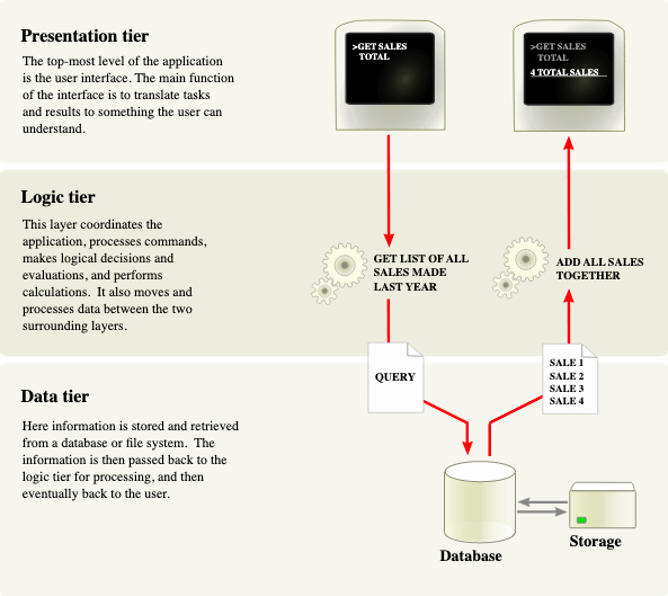
\includegraphics[width=12cm]{img/arsitekturOdoo.PNG}
	\captionof{figure}{Ilustrasi Arsitektur Odoo}
	\label{fig:asd}
\end{center}

Pada tingkatan paling atas yaitu tampilan(presentation tier), tampilan ini yang akan berinteraksi langsung dengan pengguna yang menggunakan aplikasi. Tampilan ini dibangun dengan teknologi web yaitu HTML5, Javascript, dan CSS. Tingkatan dibawahnya yaitu aturan bisnis(logic tier) yang berisi instruksi yang memproses data dan memberikan tanggapan dari interaksi kepada pengguna. Aturan pada Odoo hanya ditulis dalam bahasa pemrograman Python. Sedangkan pada tingkat paling bawah adalah tempat penyimpanan menggunakan DBMS(Database Management System), Odoo hanya bisa mendukung database PostgreSQL.\\

Odoo memiliki struktur kode yang dibentuk sebagai module untuk setiap fiturnya. Sehingga dari sisi server dan client memiliki hubungan yang disatukan menjadi satu paket tersendiri. Dimana module adalah koleksi dari fungsi dan data untuk menyelesaikan satu tujuan. Modul pada Odoo bisa ditambahkan, diganti, diubah untuk menyesuaikan kebutuhan bisnis. Dimana pada pengguna module dilambangkan dengan nama Apps, tetapi tidak semua module adalah Apps. Modules juga bisa direfrensikan sebagai addons.\\

\begingroup
\setlength{\LTleft}{-20cm plus -1fill}
\setlength{\LTright}{\LTleft}
\begin{small}
	\begin{longtable}{|p{3cm}|p{5cm}|p{5cm}|}
		\caption{Komposisi dari Module pada aplikasi Odoo}\\
		\hline
		\textbf{Elemen} & \textbf{Keterangan} & \textbf{Contoh}\\
		\endfirsthead
		
		\hline
		    Business Objects
		  & Object yang akan digunakan di module dimana setiap attribute secara otomatik dipetakan ke kolom database dengan ORM
		  & File python yang memiliki class\\
		\hline  
		Objects Views
		  & Menangani bagaimana data ditampilkan di pengguna. Seperti visualisasi form, list, kanban dan lainnya
		  & Berupa file XML dengan struktur yang sudah ditentukan Odoo\\
		\hline
		Data Files
		  & Mengelola bagaimana model data seperti laporan, konfigurasi data, data contoh dan lainnya
		  & Berupa file XML atau CSV\\
		\hline
		Web Controllers
		  & Menangani permintaan dari browser/client
		  & File python yang memiliki class namun merupakan turunan dari class odoo.http.Controller\\
		\hline
		  Static Web Data
		  & File yang digunakan hanya ditampilkan kepada client di website
		  & File gambar, File CSS, dan File JavaScript\\
		 \hline  
	\end{longtable}
\end{small}
\endgroup

Struktur database yang dibentuk pada konfigurasi umum di Odoo memiliki jumlah tabel ±566 tabel, tabel ini merupakan keseluruhan dari aplikasi dimana dapat diidentifikasi 31 tabel utama yang digunakan pada aplikasi. Berikut adalah diagram dari database yang dibuat dengan alat DBeaver Visualize, dengan attribute hanya sebuah key dari tabel. \\
\begin{center}
	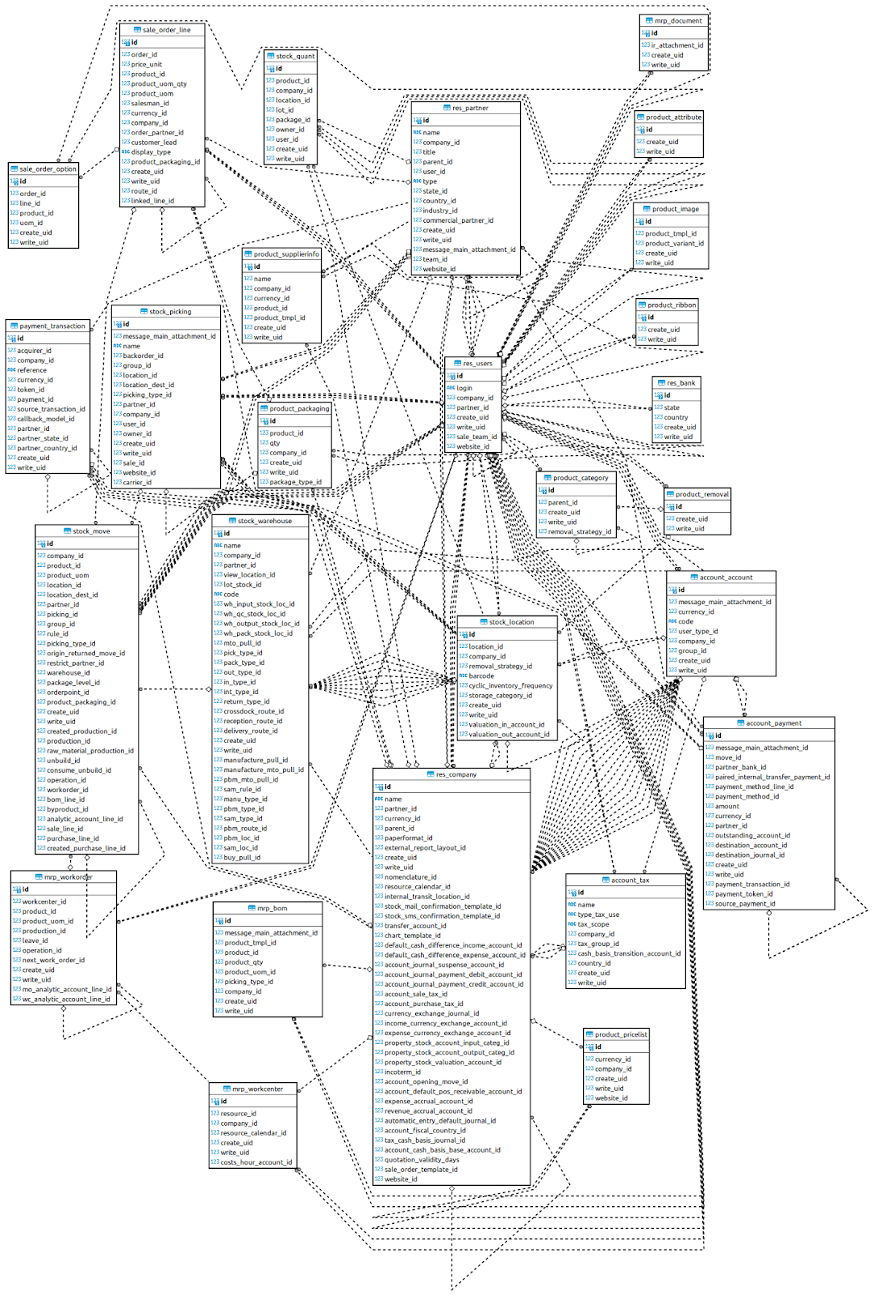
\includegraphics[width=14cm]{img/DatabaseOdoo.png}
	\captionof{figure}{Diagram Database Odoo}
	\label{fig:asd}
\end{center}



